\documentclass[11pt,a4paper]{article}

\usepackage[utf8]{inputenc}
\usepackage[T1]{fontenc}
\usepackage[spanish, es-nodecimaldot]{babel}
\addto\captionsspanish{\renewcommand{\tablename}{Tabla}}
\usepackage{geometry}
\geometry{margin=2.5cm}
\usepackage{booktabs}
\usepackage{array}
\usepackage{hyperref}
\hypersetup{colorlinks=true, linkcolor=black, urlcolor=blue}
\usepackage{parskip}
\usepackage{listings}
\usepackage{xcolor}
\usepackage{enumitem}
\usepackage{graphicx}
\usepackage{float}
\usepackage{caption}

\lstset{
  language=Java,
  basicstyle=\ttfamily\small,
  keywordstyle=\color{blue}\bfseries,
  commentstyle=\color{gray}\itshape,
  stringstyle=\color{teal},
  showstringspaces=false,
  breaklines=true,
  frame=single,
  framesep=4pt,
  xleftmargin=6pt,
  xrightmargin=6pt,
  aboveskip=6pt,
  belowskip=6pt,
}

\newcommand{\code}[1]{\texttt{#1}}
\newcommand{\file}[1]{\texttt{#1}}

\title{Refactorizaci\'on de \code{DiscretePotentialOperations}\\
       \large Descomposici\'on en clases cohesivas mediante el patr\'on Facade\\[4pt]
       \normalsize \code{org.openmarkov.core} --- paquete \code{potential.operation}}
\author{Manuel Arias Calleja}
\date{Marzo de 2026}

\begin{document}

\maketitle
\tableofcontents
\newpage

% ===================================================================
\section*{Resumen ejecutivo}

La clase \code{DiscretePotentialOperations} hab\'ia crecido con el tiempo hasta
alcanzar aproximadamente 2\,175~l\'ineas de c\'odigo, mezclando seis
responsabilidades distintas en un \'unico fichero monol\'itico: operaciones
aritm\'eticas, eliminaci\'on de variables, maximizaci\'on, fusi\'on de potenciales,
transformaciones sobre un \'unico potencial y m\'etodos de f\'abrica.  Esto
dificultaba la navegaci\'on, el testing aislado y la evoluci\'on futura del c\'odigo.

La refactorizaci\'on descrita en este documento extrae esas seis responsabilidades
en seis clases cohesivas de visibilidad de paquete, dejando
\code{DiscretePotentialOperations} como una \emph{facade} pura de unas 460~l\'ineas.
La API p\'ublica queda completamente inalterada: los 28~llamadores repartidos entre
los m\'odulos \code{core} e \code{inference} siguen compilando y pasando sus tests
sin ninguna modificaci\'on.

% ===================================================================
\section{Contexto y motivaci\'on}

\subsection{El papel de \code{DiscretePotentialOperations}}

\code{DiscretePotentialOperations} es una clase de utilidades est\'aticas que
proporciona todas las operaciones algebraicas y combinatorias primitivas sobre
valores de tipo \code{TablePotential}.  Se encuentra en el centro de cada
algoritmo de inferencia de OpenMarkov: la eliminaci\'on de variables, la
propagaci\'on de creencias, la resoluci\'on de diagramas de influencia y el
an\'alisis coste-efectividad invocan en \'ultima instancia uno o varios de sus
m\'etodos.

Por ser tan central, la clase hab\'ia ido acumulando m\'etodos a lo largo de los
a\~nos.  En el momento de esta refactorizaci\'on conten\'ia:

\begin{itemize}
  \item 28 m\'etodos p\'ublicos est\'aticos que abarcaban seis operaciones
        conceptualmente distintas.
  \item Aproximadamente 15 m\'etodos privados auxiliares, muchos de los cuales
        eran invocados por m\'etodos pertenecientes a grupos de responsabilidad
        diferentes.
  \item Una \'unica constante p\'ublica (\code{maxRoundErrorAllowed}) referenciada
        no solo internamente sino tambi\'en desde el m\'odulo \code{inference}.
  \item Un total de aproximadamente 2\,175~l\'ineas de c\'odigo.
\end{itemize}

\subsection{Problemas del dise\~no original}

\subsubsection*{Violaci\'on del Principio de Responsabilidad \'Unica}

Una clase deber\'ia tener un \'unico motivo para cambiar.
\code{DiscretePotentialOperations} ten\'ia al menos seis: un cambio en el
redondeo aritm\'etico, un cambio en la pol\'itica de desempate en la maximizaci\'on,
un cambio en la forma de fusionar potenciales\ldots\ todos ellos requerir\'ian editar
el mismo fichero, aumentando el riesgo de regresiones accidentales y dificultando
la revisi\'on del c\'odigo.

\subsubsection*{Navegabilidad deficiente}

Con 2\,175~l\'ineas, localizar la implementaci\'on de una operaci\'on concreta
exig\'ia una b\'usqueda de texto completo o conocer de memoria el orden de las
secciones dentro del fichero.  La separaci\'on por comentarios ayudaba, pero no
impon\'ia ninguna frontera estructural real.

\subsubsection*{Mezcla de niveles de abstracci\'on}

La l\'ogica de orquestaci\'on de alto nivel (por ejemplo, decidir qu\'e variables
conservar o eliminar) estaba entremezclada con la aritm\'etica de \'indices de
bajo nivel (por ejemplo, calcular los desplazamientos acumulados para recorrer
tablas multidimensionales).  El mismo m\'etodo privado
\code{findNextConfigurationAndIndexIncreasedVariable} era utilizado por las
operaciones aritm\'eticas, de eliminaci\'on, de maximizaci\'on y de fusi\'on,
creando un acoplamiento impl\'icito entre m\'etodos que conceptualmente pertenecen
a grupos distintos.

\subsubsection*{Dificultad para el testing incremental}

Al residir toda la l\'ogica en una sola clase, los tests unitarios no pod\'ian
dirigirse con facilidad a un grupo de responsabilidad sin tocar potencialmente
otro.  Los fallos en los tests eran m\'as dif\'iciles de localizar.

% ===================================================================
\section{Patr\'on de dise\~no: Facade}

\subsection{Descripci\'on del patr\'on}

El patr\'on \textbf{Facade} (Gamma et~al., \emph{Design Patterns}, 1994) proporciona
una interfaz unificada y simplificada a un subsistema de clases.  La facade no
a\~nade nueva funcionalidad; simplemente delega cada llamada a la clase de
implementaci\'on apropiada, protegiendo a los clientes de la estructura interna
del subsistema.

\begin{figure}[H]
\centering
\begin{minipage}{0.7\textwidth}
\begin{lstlisting}[language=Java, caption={Delegaci\'on t\'ipica en la Facade}]
// Public facade -- API unchanged
public final class DiscretePotentialOperations {

    public static TablePotential multiply(
            List<TablePotential> potentials) {
        return TablePotentialArithmetic.multiply(potentials);
    }

    public static TablePotential multiplyAndMarginalize(
            Collection<TablePotential> potentials,
            List<Variable> variablesToKeep,
            List<Variable> variablesToEliminate) {
        return TablePotentialElimination
                .multiplyAndMarginalize(
                        potentials,
                        variablesToKeep,
                        variablesToEliminate);
    }
    // ... 26 more delegating methods
}
\end{lstlisting}
\end{minipage}
\end{figure}

\subsection{Por qu\'e el patr\'on Facade encaja aqu\'i}

El patr\'on Facade es especialmente adecuado en esta situaci\'on por tres razones:

\begin{enumerate}
  \item \textbf{Existen 28 llamadores externos} repartidos entre dos m\'odulos
        (\code{core} e \code{inference}) que ya usan
        \code{DiscretePotentialOperations} con su nombre actual.  Renombrar o
        dividir la clase habr\'ia requerido actualizar todos esos puntos de llamada.
        La facade preserva la API existente exactamente.

  \item \textbf{La implementaci\'on es compleja y debe ocultarse.}  La aritm\'etica
        de coordenadas multidimensionales, la gesti\'on de desplazamientos y la
        l\'ogica de desempate son detalles de implementaci\'on que los llamadores
        no necesitan conocer.  La visibilidad de paquete de las clases de
        implementaci\'on impone esta encapsulaci\'on a nivel del compilador.

  \item \textbf{El subsistema tiene una descomposici\'on natural.}  Los seis grupos
        de responsabilidad identificados en la clase original se corresponden
        directamente con seis clases de implementaci\'on cohesivas.  Cada clase
        tiene un \'unico motivo para cambiar.
\end{enumerate}

\subsection{Principio complementario: Responsabilidad \'Unica}

El patr\'on Facade gestiona la \emph{interfaz externa}; el Principio de
Responsabilidad \'Unica (SRP) gobierna la \emph{descomposici\'on interna}.  Cada
una de las seis clases extra\'idas tiene exactamente una responsabilidad:

\begin{center}
\begin{tabular}{ll}
\toprule
\textbf{Clase} & \textbf{Responsabilidad} \\
\midrule
\code{TablePotentialArithmetic}   & Multiplicar, sumar, dividir, evaluar funciones \\
\code{TablePotentialElimination}  & Marginalizar, multiplicar y marginalizar \\
\code{TablePotentialMaximization} & Maximizar, multiplicar y maximizar \\
\code{TablePotentialMerge}        & Fusionar potenciales para variables de decisi\'on \\
\code{TablePotentialTransform}    & Normalizar, proyectar, corregir distribuciones \\
\code{TablePotentialFactory}      & Crear potenciales constantes, unidad o cero \\
\bottomrule
\end{tabular}
\end{center}

% ===================================================================
\section{Diagramas de clases}

\subsection{Antes de la refactorizaci\'on}

La figura~\ref{fig:antes} muestra el dise\~no original.  Una \'unica clase p\'ublica
contiene todas las operaciones aritm\'eticas, de eliminaci\'on, maximizaci\'on,
fusi\'on, transformaci\'on y f\'abrica, junto con sus m\'etodos privados auxiliares.
La \'unica otra clase del paquete relevante para este an\'alisis es
\code{AuxiliaryOperations}, que ya proporcionaba algunos auxiliares de bajo nivel.

\begin{figure}[H]
  \centering
  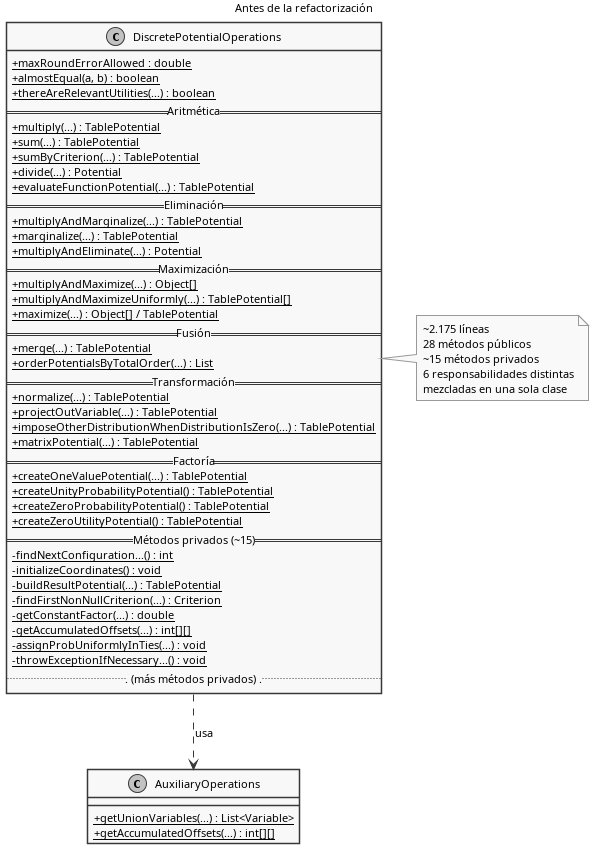
\includegraphics[width=0.55\textwidth]{antes.png}
  \caption{Diagrama de clases antes de la refactorizaci\'on.
           \code{DiscretePotentialOperations} contiene seis grupos de responsabilidad
           distintos y aproximadamente 15 m\'etodos privados auxiliares en una
           \'unica clase de 2\,175~l\'ineas.}
  \label{fig:antes}
\end{figure}

La nota del diagrama destaca los cuatro problemas principales: el tama\~no de la
clase, el n\'umero de m\'etodos p\'ublicos, los auxiliares privados que sirven a
m\'ultiples grupos no relacionados y la mezcla de seis responsabilidades
conceptualmente distintas.

\subsection{Despu\'es de la refactorizaci\'on --- estructura general}

La figura~\ref{fig:despues-estructura} muestra la estructura de alto nivel tras la
refactorizaci\'on.  \code{DiscretePotentialOperations} es ahora una \emph{facade}:
una clase de $\approx$460~l\'ineas en la que cada m\'etodo p\'ublico es una llamada
de delegaci\'on de una sola l\'inea.  Cada clase de implementaci\'on es de
visibilidad de paquete, invisible para todos los llamadores externos.

\begin{figure}[H]
  \centering
  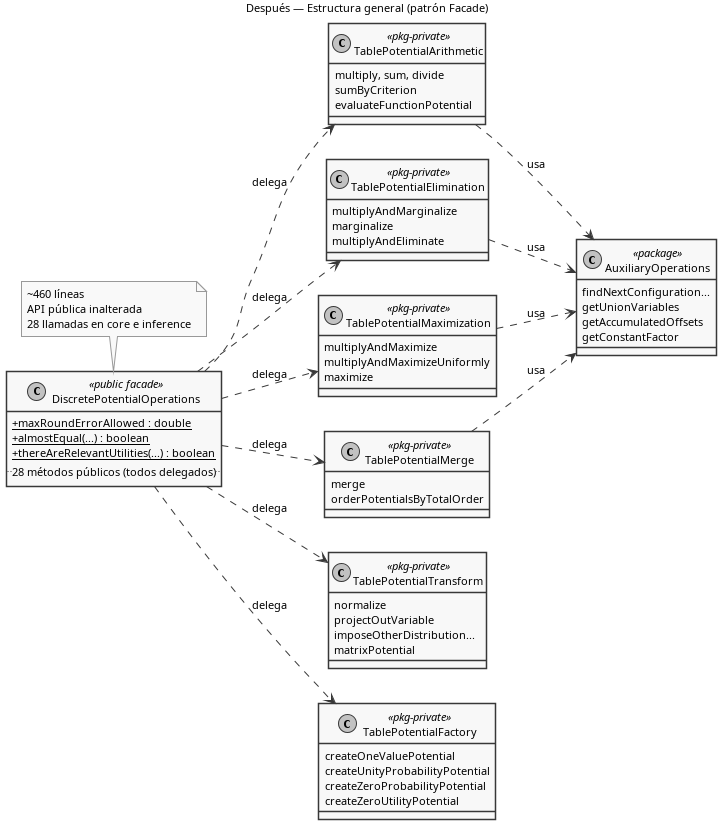
\includegraphics[width=0.65\textwidth]{despues-estructura.png}
  \caption{Estructura general tras la refactorizaci\'on.
           \code{DiscretePotentialOperations} delega en seis clases de implementaci\'on
           cohesivas con visibilidad de paquete.
           \code{AuxiliaryOperations} proporciona la aritm\'etica de \'indices
           compartida de bajo nivel.}
  \label{fig:despues-estructura}
\end{figure}

Las flechas etiquetadas con \emph{delega} representan relaciones de delegaci\'on:
la facade invoca m\'etodos de las clases de implementaci\'on, pero los llamadores
externos al paquete solo ven la facade.  Las flechas etiquetadas con \emph{usa}
representan usos ordinarios de los auxiliares compartidos en
\code{AuxiliaryOperations}.

\subsection{Despu\'es de la refactorizaci\'on --- detalle de m\'etodos}

La figura~\ref{fig:despues-detalle} muestra las firmas completas de los m\'etodos
de cada una de las seis nuevas clases con visibilidad de paquete.  Todos los
m\'etodos tienen visibilidad de paquete (\texttt{\textasciitilde}), impuesta por la
ausencia de modificador de acceso en el fuente Java, lo que significa que ninguna
clase fuera del paquete \code{potential.operation} puede invocarlos directamente.

\begin{figure}[H]
  \centering
  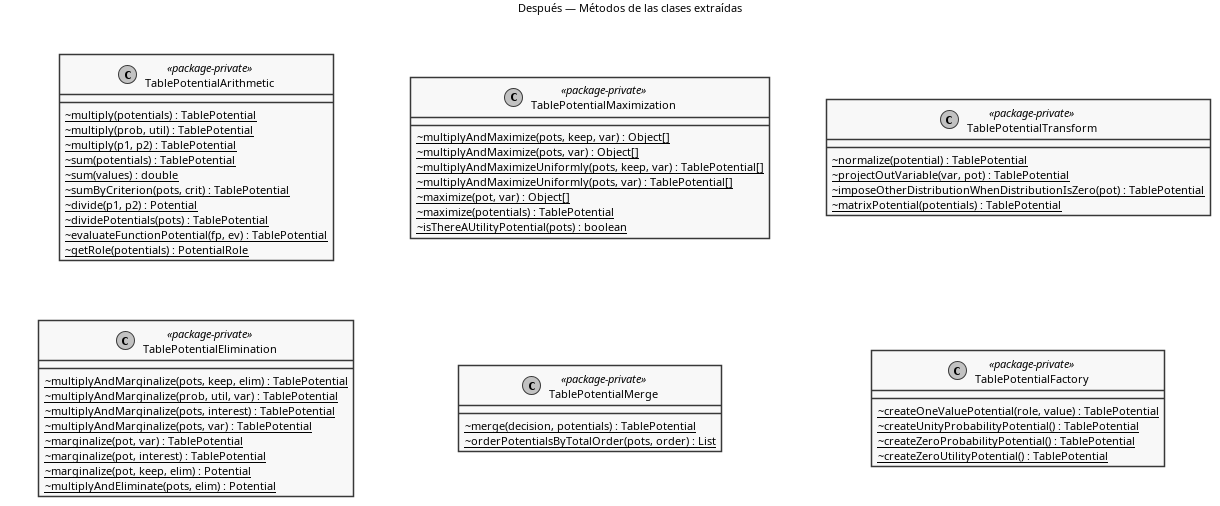
\includegraphics[width=\textwidth]{despues-detalle.png}
  \caption{Listado detallado de m\'etodos de las seis clases extra\'idas.
           El prefijo \texttt{\textasciitilde} en cada m\'etodo denota visibilidad
           de paquete.}
  \label{fig:despues-detalle}
\end{figure}

% ===================================================================
\section{Detalle de cada clase extra\'ida}

\subsection{\code{TablePotentialArithmetic}}

Esta clase contiene la l\'ogica m\'as compleja: las operaciones \code{multiply} y
\code{sum} sobre listas de \code{TablePotential} implican un bucle de incremento
de coordenadas multidimensional, gesti\'on de desplazamientos acumulados,
separaci\'on del factor constante y tratamiento de \code{StrategyTree} para
diagramas de influencia.

Tambi\'en contiene \code{evaluateFunctionPotential}, que proyecta un
\code{FunctionPotential} (definido por una expresi\'on simb\'olica) sobre una
rejilla de valores \code{TablePotential}.  Este m\'etodo se traslad\'o aqu\'i porque
comparte los mismos auxiliares privados (\code{initializeCoordinates},
\code{buildResultPotential}, \code{findFirstNonNullCriterion}) que \code{multiply}
y \code{sum}.

El auxiliar \code{getRole} determina el \code{PotentialRole} del resultado de una
operaci\'on a partir de los roles de los potenciales de entrada, y es utilizado
tambi\'en por otras clases de implementaci\'on.

\subsection{\code{TablePotentialElimination}}

Contiene cuatro sobrecargas de \code{multiplyAndMarginalize} y tres de
\code{marginalize}, cubriendo los casos habituales: eliminar una variable de un
potencial, eliminar varias variables de una lista de potenciales y la sobrecarga
especializada que multiplica un potencial de probabilidad por uno de utilidad
mientras registra las intervenciones de \code{StrategyTree}.

\code{multiplyAndEliminate} es un envoltorio de conveniencia que calcula las
variables a conservar como complemento de las variables a eliminar.

\subsection{\code{TablePotentialMaximization}}

Contiene la familia de m\'etodos \code{multiplyAndMaximize}, utilizados durante la
resoluci\'on de diagramas de influencia para calcular decisiones \'optimas.  La
sobrecarga principal construye un \code{GTablePotential<Choice>} que registra, para
cada configuraci\'on de las variables de condicionamiento, qu\'e estado de la
variable de decisi\'on alcanza la m\'axima utilidad esperada (o todos los estados
empatados, dentro de la tolerancia \code{maxRoundErrorAllowed}).

La variante \code{multiplyAndMaximizeUniformly} distribuye probabilidad
uniformemente entre los estados empatados en lugar de registrar un conjunto de
elecciones, y se utiliza al calcular pol\'iticas \'optimas aleatorizadas.

\subsection{\code{TablePotentialMerge}}

La operaci\'on \code{merge} combina una lista de potenciales (uno por estado de una
variable de decisi\'on) en un \'unico potencial cuya primera variable es la variable
de decisi\'on.  Gestiona tres flujos de datos en paralelo: los valores num\'ericos,
las intervenciones de \code{StrategyTree} y las distribuciones \code{UncertainValue}
para el an\'alisis de incertidumbre del modelo.

\code{orderPotentialsByTotalOrder} es un auxiliar utilizado por el motor de
inferencia para ordenar una lista de potenciales seg\'un un orden total dado de
variables de decisi\'on.

\subsection{\code{TablePotentialTransform}}

Re\'une las operaciones que transforman un \'unico potencial o producen uno
estrechamente relacionado:
\begin{itemize}
  \item \code{normalize}: normaliza una distribuci\'on de probabilidad condicional
        o conjunta.
  \item \code{projectOutVariable}: elimina una variable de decisi\'on de un
        potencial proyect\'andola sobre su primer estado.
  \item \code{imposeOtherDistributionWhenDistributionIsZero}: reemplaza los cortes
        de todo ceros por una masa puntual degenerada en el primer estado,
        garantizando que la normalizaci\'on posterior no divida por cero.
  \item \code{matrixPotential}: combina una lista mixta de potenciales de
        probabilidad y utilidad en un \'unico potencial (producto de probabilidades
        por suma de utilidades), usado al construir representaciones matriciales
        de decisiones.
\end{itemize}

\subsection{\code{TablePotentialFactory}}

Una clase de f\'abrica simple con cuatro m\'etodos est\'aticos para construir
instancias de \code{TablePotential} que representan valores constantes: un
potencial gen\'erico de un valor, un potencial de probabilidad unidad (valor~1 con
rol \code{CONDITIONAL\_PROBABILITY}), un potencial de probabilidad cero y un
potencial de utilidad cero.  Se usan como elementos neutros en la multiplicaci\'on,
como potenciales iniciales por defecto y en los fixtures de test.

\code{TablePotentialFactory} es la \'unica clase nueva declarada \code{public}
(en lugar de con visibilidad de paquete), ya que sus m\'etodos de f\'abrica son
invocados directamente desde varios puntos del c\'odigo fuera del paquete
\code{potential.operation}.

% ===================================================================
\section{Gesti\'on del estado compartido y dependencias entre clases}

\subsection{La constante \code{maxRoundErrorAllowed}}

La constante de tolerancia \code{maxRoundErrorAllowed} no pod\'ia trasladarse a
\code{AuxiliaryOperations} ni a \code{TablePotentialMaximization} porque es
referenciada externamente por \code{CEPotentialOperation} en el m\'odulo
\code{inference} como \code{DiscretePotentialOperations.maxRoundErrorAllowed}.
Por tanto permanece como campo \code{public static} en la facade.

\code{TablePotentialMaximization} accede a ella mediante el nombre completamente
cualificado \code{DiscretePotentialOperations.maxRoundErrorAllowed}, lo que es
correcto y deja clara la propiedad del campo.

\subsection{Auxiliares compartidos en \code{AuxiliaryOperations}}

El m\'etodo de recorrido de \'indices multidimensionales
\code{findNextConfigurationAndIndexIncreasedVariable} era un m\'etodo privado de
\code{DiscretePotentialOperations} utilizado por cuatro grupos de operaciones
diferentes.  Se traslad\'o a \code{AuxiliaryOperations} (que ya exist\'ia y
albergaba auxiliares relacionados), donde ahora es accesible para todas las clases
de implementaci\'on.  La facade conserva un envoltorio p\'ublico delegante para
garantizar la compatibilidad con cualquier llamador externo existente.

% ===================================================================
\section{Impacto en los llamadores existentes}

La refactorizaci\'on es \textbf{transparente para todos los llamadores}.  Los
28~puntos de llamada identificados antes de la refactorizaci\'on ---repartidos entre
\code{org.openmarkov.core} y \code{org.openmarkov.inference}--- no requirieron
\textbf{ninguna modificaci\'on}.  Esto se verific\'o ejecutando la suite de tests
completa de ambos m\'odulos tras cada paso de extracci\'on:

\begin{center}
\begin{tabular}{lcc}
\toprule
\textbf{M\'odulo} & \textbf{Tests} & \textbf{Fallos} \\
\midrule
\code{org.openmarkov.core}      & 337 & 0 \\
\code{org.openmarkov.inference} & 13  & 0 (3 omisiones preexistentes) \\
\bottomrule
\end{tabular}
\end{center}

% ===================================================================
\section{Ventajas del nuevo dise\~no}

\subsection{Navegabilidad}

Cada clase tiene un nombre autodescriptivo.  Un desarrollador que busca la l\'ogica
de marginalizaci\'on abre \code{TablePotentialElimination.java}; uno que depura un
problema de maximizaci\'on abre \code{TablePotentialMaximization.java}.  Ya no
hace falta desplazarse por 2\,000~l\'ineas para encontrar el c\'odigo relevante.

\subsection{Responsabilidad \'unica y cohesi\'on}

Cada una de las seis clases nuevas tiene un \'unico motivo para cambiar.  Una
modificaci\'on en la pol\'itica de desempate de \code{multiplyAndMaximize} queda
contenida \'integramente en \code{TablePotentialMaximization}, sin riesgo de
afectar accidentalmente a la l\'ogica aritm\'etica o de eliminaci\'on.

\subsection{Encapsulaci\'on forzada}

La visibilidad de paquete de las clases de implementaci\'on implica que ning\'un
c\'odigo externo al paquete \code{potential.operation} puede depender directamente
de ellas.  Todo acceso externo debe pasar por la facade, que ofrece una interfaz
estable y documentada.

\subsection{Testabilidad}

Al estar cada clase centrada en una \'unica preocupaci\'on, es posible escribir
tests unitarios que apunten exactamente a una clase de implementaci\'on.  Un test
para \code{TablePotentialElimination} no necesita tener en cuenta la l\'ogica de
maximizaci\'on ni de fusi\'on, lo que simplifica los tests y facilita el
diagn\'ostico de fallos.

\subsection{Reducci\'on de la carga cognitiva}

La mayor de las seis clases nuevas, \code{TablePotentialArithmetic}, tiene
aproximadamente 450~l\'ineas, comparable al tama\~no de la \emph{nueva} facade.
Ning\'un fichero supera las 400--450~l\'ineas, lo que mantiene cada fichero dentro
de un rango que un desarrollador puede leer c\'omodamente en una sola sesi\'on.

\subsection{Evoluci\'on futura m\'as sencilla}

Los cambios futuros ---como a\~nadir aritm\'etica acelerada por GPU o un nuevo tipo
de operaci\'on sobre potenciales--- pueden realizarse modificando o extendiendo una
\'unica clase cohesiva, a\~nadiendo un m\'etodo delegante a la facade y escribiendo
tests dirigidos.  El impacto de ese cambio queda limitado a un m\'aximo de dos
ficheros.

% ===================================================================
\section{Resumen de los cambios}

\begin{center}
\begin{tabular}{lrl}
\toprule
\textbf{Fichero} & \textbf{L\'ineas} & \textbf{Cambio} \\
\midrule
\code{DiscretePotentialOperations.java} & $\approx$460 & Reducida a facade; eliminadas 3 constantes muertas \\
\code{AuxiliaryOperations.java}         & ampliada     & A\~nadidos 4 m\'etodos procedentes de \code{DPO} \\
\code{TablePotentialArithmetic.java}    & $\approx$450 & Nueva clase (visibilidad de paquete) \\
\code{TablePotentialElimination.java}   & $\approx$325 & Nueva clase (visibilidad de paquete) \\
\code{TablePotentialMaximization.java}  & $\approx$400 & Nueva clase (visibilidad de paquete) \\
\code{TablePotentialMerge.java}         & $\approx$280 & Nueva clase (visibilidad de paquete) \\
\code{TablePotentialTransform.java}     & $\approx$150 & Nueva clase (visibilidad de paquete) \\
\code{TablePotentialFactory.java}       & $\approx$55  & Nueva clase (p\'ublica) \\
\bottomrule
\end{tabular}
\end{center}

\end{document}
